\documentclass[border=3mm]{standalone}
\usepackage{amsmath,amssymb,pgfplots}
\usepgfplotslibrary{groupplots}
\pgfplotsset{compat=1.18}

\definecolor{evalteal}{HTML}{087F8C}
\definecolor{evalnavy}{HTML}{17324D}
\definecolor{evalgray}{HTML}{97A3B1}
\definecolor{evalorange}{HTML}{B95C16}

\begin{document}
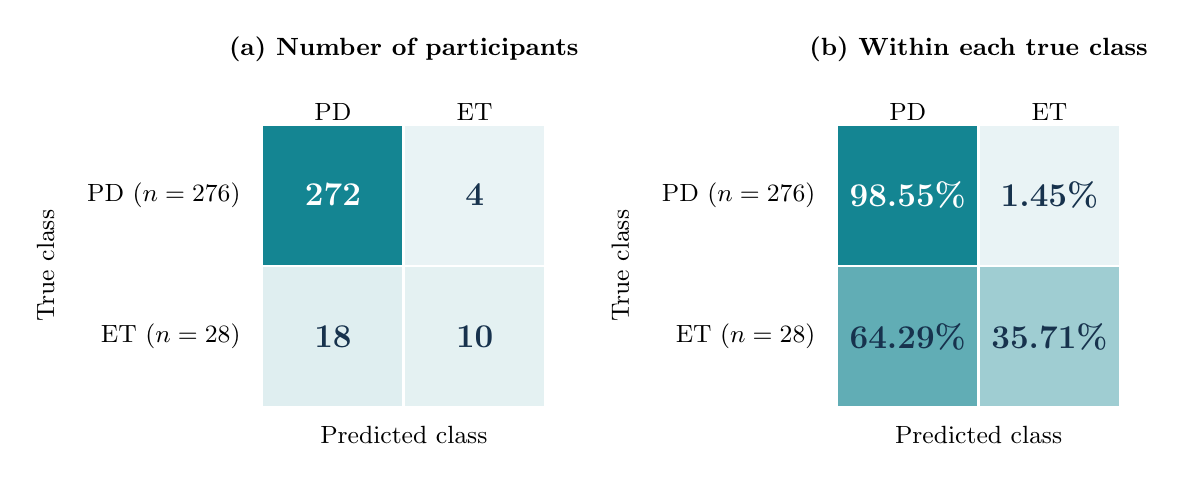
\begin{tikzpicture}[font=\small]
\begin{scope}[xshift=0.0cm]
\node[font=\small\bfseries] at (2.75,0.8) {(a) Number of participants};
\node at (1.85,0) {PD};
\node at (3.6500000000000004,0) {ET};
\node[anchor=east] at (0.8,-1.05) {PD ($n=276$)};
\filldraw[fill=evalteal!95!white,draw=white,line width=1pt] (0.9500000000000001,-1.9500000000000002) rectangle (2.75,-0.15000000000000002);
\node[text=white,font=\large\bfseries] at (1.85,-1.05) {272};
\filldraw[fill=evalteal!9!white,draw=white,line width=1pt] (2.7500000000000004,-1.9500000000000002) rectangle (4.550000000000001,-0.15000000000000002);
\node[text=evalnavy,font=\large\bfseries] at (3.6500000000000004,-1.05) {4};
\node[anchor=east] at (0.8,-2.85) {ET ($n=28$)};
\filldraw[fill=evalteal!13!white,draw=white,line width=1pt] (0.9500000000000001,-3.75) rectangle (2.75,-1.9500000000000002);
\node[text=evalnavy,font=\large\bfseries] at (1.85,-2.85) {18};
\filldraw[fill=evalteal!11!white,draw=white,line width=1pt] (2.7500000000000004,-3.75) rectangle (4.550000000000001,-1.9500000000000002);
\node[text=evalnavy,font=\large\bfseries] at (3.6500000000000004,-2.85) {10};
\node at (2.75,-4.1) {Predicted class};
\node[rotate=90] at (-1.8,-1.95) {True class};
\end{scope}
\begin{scope}[xshift=7.3cm]
\node[font=\small\bfseries] at (2.75,0.8) {(b) Within each true class};
\node at (1.85,0) {PD};
\node at (3.6500000000000004,0) {ET};
\node[anchor=east] at (0.8,-1.05) {PD ($n=276$)};
\filldraw[fill=evalteal!95!white,draw=white,line width=1pt] (0.9500000000000001,-1.9500000000000002) rectangle (2.75,-0.15000000000000002);
\node[text=white,font=\large\bfseries] at (1.85,-1.05) {98.55\%};
\filldraw[fill=evalteal!9!white,draw=white,line width=1pt] (2.7500000000000004,-1.9500000000000002) rectangle (4.550000000000001,-0.15000000000000002);
\node[text=evalnavy,font=\large\bfseries] at (3.6500000000000004,-1.05) {1.45\%};
\node[anchor=east] at (0.8,-2.85) {ET ($n=28$)};
\filldraw[fill=evalteal!64!white,draw=white,line width=1pt] (0.9500000000000001,-3.75) rectangle (2.75,-1.9500000000000002);
\node[text=evalnavy,font=\large\bfseries] at (1.85,-2.85) {64.29\%};
\filldraw[fill=evalteal!39!white,draw=white,line width=1pt] (2.7500000000000004,-3.75) rectangle (4.550000000000001,-1.9500000000000002);
\node[text=evalnavy,font=\large\bfseries] at (3.6500000000000004,-2.85) {35.71\%};
\node at (2.75,-4.1) {Predicted class};
\node[rotate=90] at (-1.8,-1.95) {True class};
\end{scope}
\end{tikzpicture}
\end{document}
